\subsection{Solar Activity Period Estimation}
We can see from figure \ref{fig:monthly_temp} that there is no clear trend or period in the data. It is worth pointing out that there are no values at 1 or 0 which would be expected from normalized data as the data has been averaged.

\begin{figure}[H]
    \centering
%    \begin{subfigure}[b]{0.48\textwidth}
        \centering
        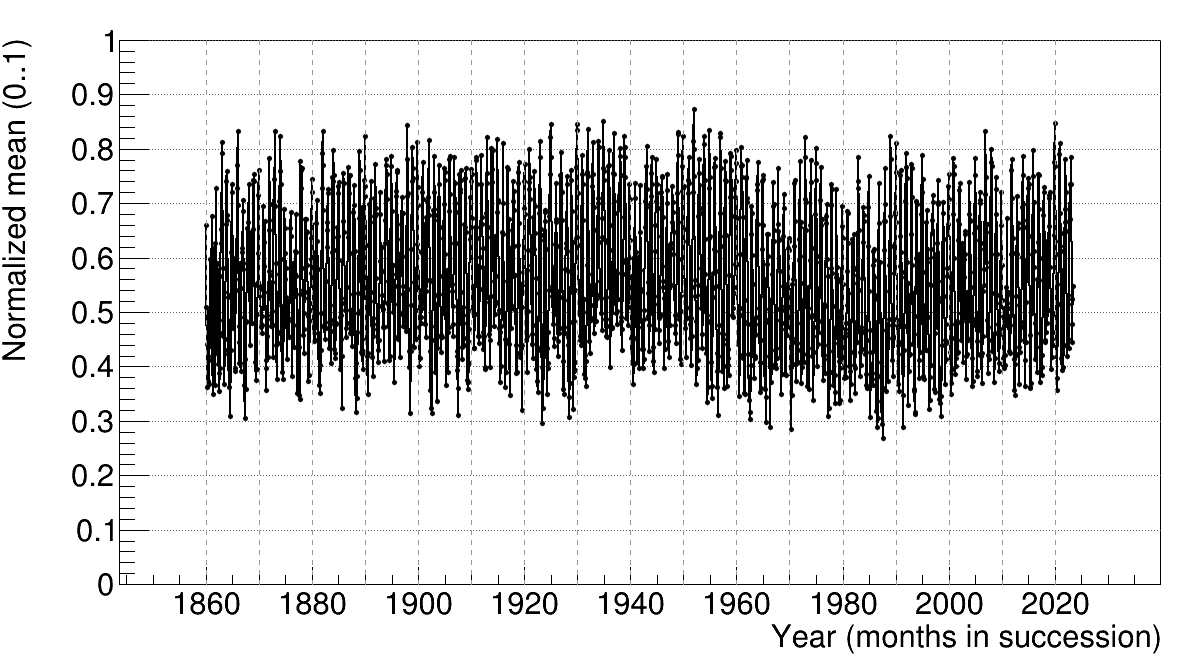
\includegraphics[width=0.9\textwidth]{../plots/solar/monthly_norm_temp_timeline.png}
        \caption{This graph shows the normalized monthly temperature averaged for each month plotted in succession.}
        \label{fig:monthly_temp}
%    \end{subfigure}
\end{figure}
To be able to see what frequencies are actually relevant a fast fourier transform was done and the frequencies are plotted in \ref{fig:freq}.

\begin{figure}[H]
%    \begin{subfigure}[b]{0.48\textwidth}
        \centering
        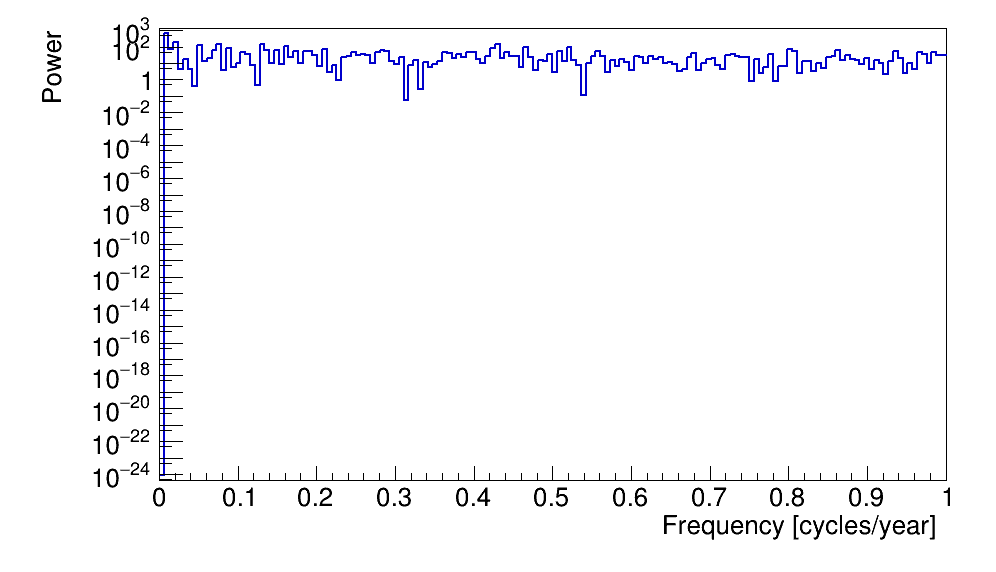
\includegraphics[width=0.9\textwidth]{../plots/solar/solar_frequency_analysis.png}
        \caption{This graph shows the most relevant frequencies in the data from \ref{fig:monthly_temp}.}
        \label{fig:freq}
\end{figure}


To be able to more clearly see the actual periods, we inverted this graph to show information more clearly.

\begin{figure}[H]
    \centering
    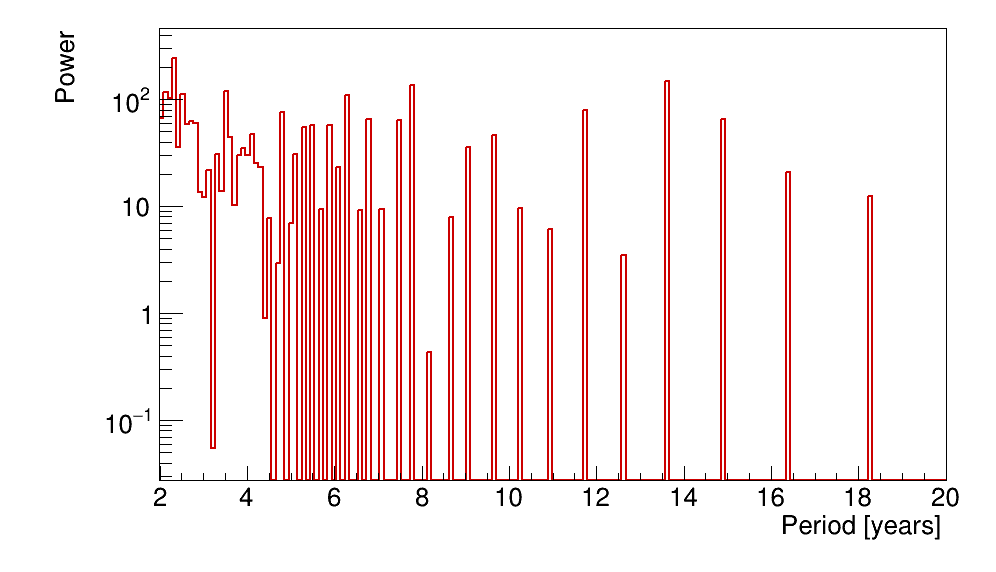
\includegraphics[width=0.9\textwidth]{../plots/solar/period_analysis.png}
    \caption{periods of data in the \ref{fig:freq} graph.}
    \label{fig:period}
\end{figure}

\subsubsection{Discussion}

It is quite clear to see the data is not great. There is a lot of noise and none of the frequencies really stand out. It can quickly be looked up that the period of solar activity is around 11 years, and while \ref{fig:period} shows a peak there, the peak is pretty weak compared to everything else. This can also be seen in the \ref{fig:freq} as the frequency graph looks pretty much like a step function, with some noise. This disagrees with the original expectation that this time series would have a peak frequency in line with the known solar activity frequency.

To improve this study in the future a lot of things need to be done. Firstly data should be taken from more places around the world rather than limited to Sweden. Also meteorological effects should be taken into account as a cloudy day could mess with the data. Additionally rather than averaging every month, it may be more insightful to use a smoothing algorhithm on the data as that would remove some of the high frequency noise. Also the other sources of noise should be understood to be eliminated

\subsubsection{Conclusion}

Data disagrees with the research Question which means that either the solar cycle cannot be estimated using the temperature data, more data is needed, or data needs to be processed to a higher standard. There was a peak present at the expected 11 years, but it wasn't a major peak, indicating that it was not the most relevant in the datas frequencies.